\chapter{Introduction}

MeDSpace D2RMap is a declarative language to describe mappings between relational database schemas and OWL ontologies. The language is a derived work of the D2R Map language designed by Chris Bizer \cite{D2RMap}. As D2RMap is licensed under GNU LGPL v.2.1, this derived work is also licensed under GNU LGPL v.2.1 
\footnote{\url{http://www.gnu.de/documents/lgpl-2.1.en.html}}. 

MeDSpace D2RMap is tailored to the needs for the MeDSpace dataspace and thus some language features were removed from the original D2RMap language and other features  were added.

This document defines the syntax and semantics of the MeDSpace D2R Map language and mentions the
changes in regards to the original D2R Map language where it is needed.

The next section is basically adopted from the original D2R Map language specification \footnote{\url{http://wifo5-03.informatik.uni-mannheim.de/bizer/d2rmap/D2R\_language\%20specification.pdf}}
. The concepts have barely changed, only the language terminology and some details have changed.

\section{The D2R Mapping Process}

The D2R mapping process executed by the D2R wrapper has four logical steps:

\begin{enumerate}  
	\item Selection of a record set from the database using SQL 
	\item Grouping of the record set by the \textit{resourceIdColumns} \footnote{resourceIDColumns is an attribute of the d2r:ClassMap element}
	columns. 
	\item Creation of class instances and identifier construction. 
	\item Mapping of the grouped record set data to instance properties.
\end{enumerate}

\begin{figure}[H]
	\begin{center}
		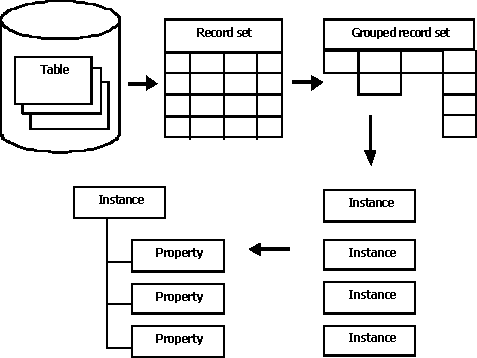
\includegraphics [width=0.75\textwidth]{../images/MappingProcess.pdf}
	\end{center}
	\caption{The MeDSpace D2R mapping process}
	\label{MappingProcessFigure}
\end{figure}

For each class or group of similar classes a record set is selected from the
database. Second, the record set is grouped according to the resourceIDColumns columns of
the specific d2r:ClassMap. Then the class instances are created and assigned an URI identifier. Blank Node creation is currently not supported, as it is not needed in the MeDSpace dataspace. Finally, the instance properties are created using
datatype and object property bridges.
The division between step three and four allows references to other instances dynamically created in the mapping process.

\chapter{Language Specification}

A MeDSpace D2R Map is a well-formed XML document. It's structure is defined by the accompanying \textit{Medspace{\_}D2RMap.xsd} file. The elements of the MeDSpace D2R Map belong to the namespace
\begin{center}
	\textbf{http://www.medspace.com/D2Rmap}
\end{center}

\section{Root Element: Root}
\textbf{Description:} \newline
Root element of the d2r mapping.

\textbf{Attributes:} \newline
\BeginAttribute[xmlns, \emph{required}]
MeDSpace D2R namespace declaration.
\EndAttribute

\textbf{Sub Elements:} \newline
\BeginAttribute[DBConnection, \emph{required}]
Has to occur has the first element and it may occur only once. 
\EndAttribute
\BeginAttribute[Namespace, \emph{optional}]
Can occur any number of times
\EndAttribute
\BeginAttribute[ClassMap, \emph{optional}]
Can occur any number of times
\EndAttribute

\begin{ExampleBox}
	<d2r:Root xmlns:d2r="http://www.medspace.com/D2Rmap">
		\begin{indention}{1cm}
		\XMLComment{DBConnection element is required} \\		
		\XMLComment{Than follows an optional list of namespaces and class maps in any order}\\
		
		\end{indention}
	</d2r:Root>
\end{ExampleBox}


\section{Top-Level-Elements}

\subsection{DBConnection}
\textbf{Description:} \newline
Defines properties to specify and customize the connection to a relational database

\textbf{Attributes:} \newline
\BeginAttribute[jdbcDriver, \emph{required}]
The jdbc driver to use for opening a jdbc connection to the database.
\EndAttribute
\BeginAttribute[jdbcDSN, \emph{required}]
The jdbc Data Source Name, i.d. the URI to address the database.
\EndAttribute
\BeginAttribute[poolSize, \emph{optional}]
The maximum size of the connection pool, the wrapper should use. If not specified a default value is used.
\EndAttribute

\textbf{Sub Elements:} \newline
\BeginAttribute[DBAuthentification, \emph{optional}]
If it occurrs, it has to be stated has the first sub element.
Can only occur once.
\EndAttribute
\BeginAttribute[DataSourceProperty, \emph{optional}]
A property for the datasource. Can occur in any number of times.
\EndAttribute

\begin{ExampleBox}
	<d2r:DBConnection
	\begin{indention}{1cm}
		jdbcDriver="com.mysql.jdbc.Driver"\\
		jdbcDSN="jdbc:mysql://localhost:3306/medspace?useSSL=false"\\
		poolSize=10
	\end{indention}
	>
		\begin{indention}{1cm}
		\XMLComment{DBAuthentification element is required}\\
		\XMLComment{Than follows an optional list of datasource properties}
		\end{indention}
	</d2r:DBConnection>
\end{ExampleBox}

\subsubsection{DBAuthentification}
\textbf{Description:} \newline
DBAuthentification is used to authenticate in the database with username and password

\textbf{Attributes:} \newline
\BeginAttribute[username, \emph{required}]
The user name needed for database authentification.
\EndAttribute
\BeginAttribute[password, \emph{optional}]
The password needed for database authentification.
\EndAttribute

\begin{ExampleBox}
	<d2r:DBAuthentification
	\begin{indention}{1cm}
		username="root"\\
		password="1234"	
	\end{indention}
	/>
\end{ExampleBox}

\subsubsection{DataSourceProperty}
\textbf{Description:} \newline
Describes a datasource specific property, that is send to the datasource while establishing a connection to it.

\textbf{Attributes:} \newline
\BeginAttribute[name, \emph{required}]
The name of the property.
\EndAttribute
\BeginAttribute[value, \emph{required}]
The value of the property.
\EndAttribute

\begin{ExampleBox}
	<d2r:DataSourceProperty name="cacheResultSetMetadata" value="true"/>
\end{ExampleBox}


\subsection{Namespace}
\textbf{Description:} \newline
Defines a RDF namespace the wrapper can use.

\textbf{Attributes:} \newline
\BeginAttribute[prefix, \emph{required}]
The prefix to use in the rdf triples.
\EndAttribute
\BeginAttribute[namespace, \emph{required}]
The namespace represented by the prefix.
\EndAttribute

\begin{ExampleBox}
	<d2r:Namespace 
	\begin{indention}{1cm}
		prefix="rdf"\\
		namespace="http://www.w3.org/1999/02/22-rdf-syntax-ns\#"
	\end{indention}
	/>
\end{ExampleBox}

\subsection{ClassMap}
\textbf{Description:} \newline
A ClassMap maps a virtual view of SQL table data to rdf triples. The view is defined by a regular SQL query.

\textbf{Attributes:} \newline
\BeginAttribute[type, \emph{required}]
the type (rdf:type) for the mapped data.
\EndAttribute
\BeginAttribute[id, \emph{required}]
Assigns a unique id to the ClassMap. The is can be used by other ClassMaps to refer this ClassMap.
\EndAttribute
\BeginAttribute[baseURI, \emph{required}]
a prefix used to generate the URI of the mapped sql data.
\EndAttribute
\BeginAttribute[resourceIdColumns, \emph{required}]
Specifies the columns of the sql query, which are used along with the base URI for generating the URI of rdf triples.
\EndAttribute
\BeginAttribute[sql, \emph{required}]
A sql query, that specifies the sql data, that should be mapped.
\EndAttribute

\textbf{Sub Elements:} \newline
\BeginAttribute[DataTypePropertyBridge, \emph{optional}]
Defines a new datatype property bridge. Can occur in any number of times.
\EndAttribute
\BeginAttribute[ObjectPropertyBridge, \emph{optional}]
Defines a new object property bridge. Can occur in any number of times.
\EndAttribute
\BeginAttribute[MetaData, \emph{optional}]
Adds searchable meta data tags. Tags have to be separated by spaces.
\EndAttribute
\begin{ExampleBox}
	<d2r:ClassMap 
	\begin{indention}{1cm}
		type="test:patient"\\
		sql="SELECT p.id, p.dateOfBirth, p.sex, p.maritalstatus, p.language\\ 
		FROM patient p;"\\
		resourceIdColumns="patient.id"\\
		baseURI="http://www.example.com/patient\#"\\
		id="patient"
	\end{indention}
	>

	\begin{indention}{1cm}
		\XMLComment{Optional list of DataTypePropertieBridge instances}\\
		\XMLComment{Optional list of ObjectPropertyBridge instances}\\
		\XMLComment{Optional list of MetaData instances}
	\end{indention}	
	
	</d2r:ClassMap>
\end{ExampleBox}

\section{Property Mappings}
Property mappings define bridges between columns of the result set and instance
properties.

If a value in the result set is NULL, no property of the specific type is defined for
that instance.

\subsection{DataTypePropertyBridge}
\textbf{Description:} \newline
A DatatypePropertyBridge defines a bridge between a column of the result set and a literal property of the instances created.

\textbf{Attributes:} \newline
\BeginAttribute[property, \emph{required}]
The name of the rdf property
\EndAttribute
\label{patternLabel}
\BeginAttribute[pattern, \emph{required}]
Defines the value of the property. It is possible to use the content of the sql tuple: The content of a column of a SQL query (defined by the ClassMap the property bridge belongs to) can be accessed by beginning with '@@' than writing the column in the format t.c (where t is the table name and c is the column name) and than ending the expression with '@@'.

\emph{Example:}\newline
If 'patient' is a table and 'name' is a column of 'patient', than the content of 'name' can be accessed by '@@patient.name@@'

\emph{Note:} \newline
Aliases can be used. If m is an alias for maritalstatus, @@m.name@@ is the same as maritalstatus.name
\EndAttribute
\BeginAttribute[dataType, \emph{optional}]
Specifies a rdf datatype for the property.
\EndAttribute
\BeginAttribute[lang, \emph{optional}]
Specifies a language tag,e.g. "de" or "en", for the property.
\EndAttribute

\begin{ExampleBox}
	<d2r:DataTypePropertyBridge 
	\begin{indention}{1cm}
		property="test:languageName"\\
		pattern="@@language.name@@"\\ 
		dataType="rdf:langString"\\
		lang="en"
	\end{indention}
	/>
\end{ExampleBox}

\subsection{ObjectPropertyBridge}
\textbf{Description:} \newline
ObjectPropertyBridge defines a bridge between a column of the result set and an rdf resource of the created instances.

\textbf{Attributes:} \newline
\BeginAttribute[property, \emph{required}]
The uri (qualified name) of the rdf property
\EndAttribute
\label{refferedClassLabel}
\BeginAttribute[referredClass, \emph{optional}] 
Specifies, that this bridge refers to a resource of another ClassMap. 
The value of this attribute is the id of the referred ClassMap.
\EndAttribute
\BeginAttribute[referredColumns, \emph{optional}]
This attribute is only used, if the attribute \emph{referredClass} is used.
This attribute specifies the columns in the sql query (from the ClassMap this property belongs to and not the referred ClassMap), that define the referred rdf resource. The columns should match the attribute "resourceIdColumns" of the referred ClassMap in order ensure to produce valid rdf resource references. This is important, as there is no automatic validation. The User is responsible for specifying the right columns in the right order.
\EndAttribute
\BeginAttribute[pattern, \emph{optional}]
Specifies, that instead of a ClassMap references a general pattern should be used. See the DataTypePropertyBridge \hyperref[patternLabel]{\emph{pattern}} 
for more details about the pattern generation.

Note:\newline
This attribute will be ignored, if the
\hyperref[refferedClassLabel]{\emph{refferedClass}} attribute is specified.
\EndAttribute

\begin{ExampleBox}
	<d2r:ObjectPropertyBridge 
	\begin{indention}{1cm}
		property="test:maritalstatus"\\
		pattern="maritalstatus\_namespace:@@patient.maritalstatus@@"
	\end{indention}
	/>
	
	\XMLComment{The same object property, but using the referredClass attribute; This example assumes, that there exists a ClassMap having the id \emph{maritalstatus}}\\
	<d2r:ObjectPropertyBridge 
	\begin{indention}{1cm}
		property="test:maritalstatus"\\
		referredClass="maritalstatus"\\
		referredColumns="patient.maritalstatus"
	\end{indention}
	/>
\end{ExampleBox}


\subsection{MetaData}
\textbf{Description:} \newline
MetaData is a searchable meta data tag. It is possible to state several tags. Each tag is thereby
separated by a space.


\begin{ExampleBox}
	<d2r:MetaData>tag1 tag2</d2r:MetaData> 
\end{ExampleBox}